\chapter{Constructing the Social network}

The driving fuel for any social network is the data it represents. The problem in constructing a linked-data system such as this one is always the data and the entropy it brings with itself. The challenges are always the usual ones - unavailability of data, noise in the collected data, no authentic source, and many-a-times no structure in the data. Even if we are successful in collecting and cleaning the linked data we want, the way we go about integrating all this variety of information in a single data store is itself an another challenge. \\

The choice of data store matters here the most because one would like to query the data and unearth interesting relations between participating entities. Henceforth, a person or an organization will be called an entity. These entities would be linked to each other by certain edges/links just like in a graph which we will normally call relations. All these challenges are elevated manifold when one wishes to resolve entities from different datasets into a single unified entity. \\

Here we describe in order our choice of data storage, our core data model for the linked data, data collection practices and data sources, data integration methodology, and finally the necessary evil in such a system -  entity resolution. \\

\section{Everything is a graph}
\label{datamodel}
We begin by describing how we are going to actually store any kind of linked data we get and why our approach is a sensible one. We describe here where our core data is stored and how our core data model looks like. It has to be stated at the onset that care has been taken to ensure that
whatever data goes in our core data modal is non-redundant, free of noise and verified. As already stated, our goal is to construct a social network between politicians, companies, entrepreneurs, military personnel, bureaucrats, political parties, universities, movie actors, and any important entity one can think of in the usual power hierarchy. Also, we want to be able to model all kinds of relationships that can exist between these entities with ease: family-links, donation-links, director-links, ownership-links, subsidiary-links, etc. \\

Practically anything connected can be represented by a graph. We live in a connected world. There are no isolated pieces of information, but rich, connected domains all around us. Thus, it makes sense to model our core data as a large inter-connected graph where every node is an entity and every edge represents a link between two of them.   \\

% (or a hyper-graph to be exact, refer our LIMITATIONS section)


A graph is composed of two elements: a node and a relationship. Each node represents an entity (a person, place, thing, category or other piece of data), and each relationship represents how two nodes are associated. This general-purpose structure allows you to model all kinds of scenarios - from a system of roads, to a network of devices, to a population's medical history or anything else defined by relationships.  \\

Before beginning to describe how we achieve the above, it is important to understand that even traditional SQL tables are a connected piece of information, and can be modeled using a graph. \\

What we provide is therefore a graph to the user where he fits any relevant connected data he has. The choice of the data model is clear, but two problems remain - how we are going to store our graph's interconnected data, and how do we query it efficiently for digging out interesting relationships. Our next two sections discuss the same. \\

\subsection{Neo4j}

Neo4j \cite{neo}  is our choice of data storage. It is one of the leading JVM based NoSQL graph databases. We build our knowledge base on it as a graph and thus Neo4j is at the center of our entire system. We chose Neo4j because of the following reasons , and we have found it be a non-separable asset to our use cases. \cite{neogdb} \\

\begin{enumerate}

\item Only a database that embraces relationships as a core aspect of its data model is able to store, process, and query connections efficiently. While other databases compute relationships expensively at query time, a graph database stores connections as first class citizens, readily available for any 'join-like' navigation operation. Accessing those already persistent connections is an efficient, constant-time operation and allows you to quickly traverse millions of connections per second per core. 

\item Graph databases are designed to mimic the most natural way we tend to model data - the same way you would map it all out on a white-board. Your collection of circles, boxes, lines and arrows is - in essence - already a graph. 

\item In Neo4j, everything is stored in form of either an edge, a node or an attribute. Each node and edge can have any number of attributes. Both the nodes and edges can be labeled. Labels can be used to narrow searches.  Neo4j is very easy to learn and adapt. It's object property model is very intuitive and anything can be modeled on a white board in the form of nodes and edges.

\item Constant time traversals for relationships in the graph both in depth and in breadth due to efficient representation of nodes and relationships 

\item All relationships in Neo4j are equally important and fast, making it possible to materialize and use new relationships later on to 'shortcut' and speed up the domain data when new needs arise 

\item Compact storage and memory caching for graphs, resulting in efficient scale-up and billions of nodes in one database on moderate hardware 

\item It's NoSQL help us in modeling the varied data from different sources we have collected.

\item The cypher query language provided by Neo4j helps in querying the connected data very easily and is very powerful. Also, the Neo4j browser client provided by Neo4j is very good for visualizing the results of the cypher queries.

\end{enumerate}

That said, it is important to note that Google uses Cayley - an open source graph database -  to power it's google's knowledge graph.\cite{cayley} 


\subsection{Property Graph Model Explained}

Let us dive into some examples which explain how me model our core data in Neo4j using it's property graph model.\cite{neogdb}  \\

\begin{enumerate}

\item The property graph contains connected entities (the nodes) which can hold any number of attributes (key-value-pairs). What this means for us is: a person node can have different attributes his date-of-birth, address, email, sex, etc.

\item Nodes can be tagged with labels representing their different roles in our domain. That said, this unique thing about Neo4j helps us in specifying IS-A relationships via multiple labels on a single Neo4j node. Thus, a node can be labeled as a person, politician, businessman at the same time. The same information is very hard to model in traditional SQL databases.

\item In addition to contextualizing node and relationship properties, labels may also serve to attach meta-data index or constraint information to certain nodes.

\item Relationships provide directed, named semantically relevant connections between two node-entities. A relationship always has a direction, a type, a start node, and an end node. This model is exactly the same as directed edges in a traditional graph structure. Although they are directed, relationships can always be navigated regardless of direction.

\item A relationship can also be labeled by a single label specifying what kind of a relationship exists between two nodes. Thus, if a politician is 'son-of' a businessman we can connect the two nodes by an edge attributed with such a label.

\item Just like a node, a relationship can also hold any number of attributes(key-value pairs). In most cases, relationships have quantitative properties, such as weights, costs, distances, ratings, time intervals, or strengths. 

% But for our use case, one can think of an example relationship as : a particular `person`(node) 'donated'(relationship-type) 'x amount of money at y date'(relationship properties) to(directed edge) a particular `politician`(node).

\item As relationships are stored efficiently, two nodes can share any number or type of relationships without sacrificing performance.

\end{enumerate}

An example could be the Figure \ref{fig:neo1}

\begin{figure}[H]
\begin{center}  
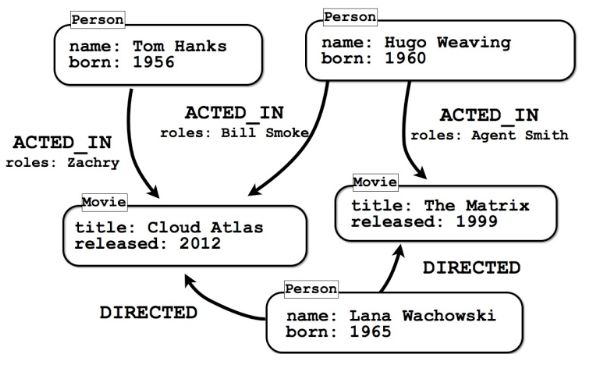
\includegraphics[width=0.7\textwidth]{neo1} 
\caption{An example of property graph model}
\label{fig:neo1}
\end{center}
\end{figure}

\subsection{Cypher}

Cypher is a declarative graph query language for the graph database Neo4j that allows for expressive and efficient querying and updating of the graph store. Cypher is a relatively simple but still very powerful language. Very complicated database queries can easily be expressed through Cypher. This allows users to focus on their domain instead of getting lost in database access. \\

A node is represented like this: \\
    \emph{(:person:politician {name:\textbf{'Narendra Modi'},sex:'M'})}\\ \\
A relation is represented like this:\\
    \emph{(startnode)-[:relatedto {kind:\textbf{'childof'}}]-$\textgreater$(endnode)}\\ \\
The structure here is self explanatory and can be further explored by reading Neo4j manual. Figure \ref{fig:neo2} explains better.


\begin{figure}[H]
\begin{center}  
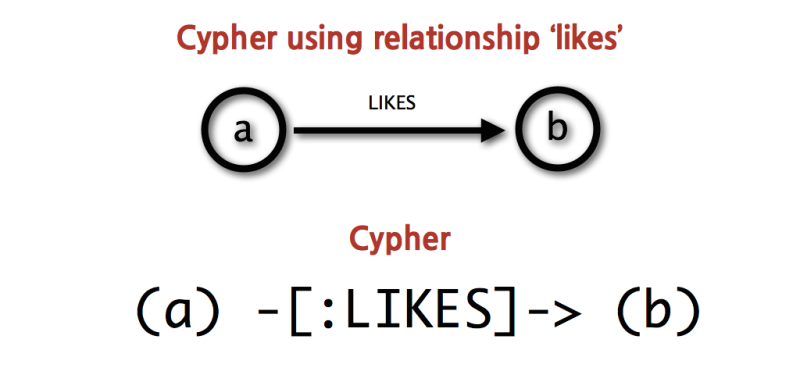
\includegraphics[width=0.7\textwidth]{neo2} 
\caption{Cypher Example}
\label{fig:neo2}
\end{center}
\end{figure}


Querying in cypher is as easy as thinking about how you traverse a graph. Here is a simple query to return all the relationships that start from or end at node 'Naveen Jindal' of type politician.

\emph{ \textbf{MATCH} (jindal:politician {name:\textbf{'Naveen Jindal'}})-[anyrelation]-(anynode)
 \textbf{RETURN} anyrelation }

Interested readers can be direct here to read more about cypher in Neo4j's manual\cite{neomanual}: 
\subsection{Our restricted property graph model}

We had to specify some ground rules to model our data for imposing uniformity on varied data that is being fed into the system. Thus, our property data model follows the rules stated below.

\begin {enumerate}

\item As allowed by Neo4j - a node can have more than one label, a relation always has only one label.

\item Every node and a relation has a unique uuid/relid.

\item All nodes are labeled 'entity' by default. To make anonymous queries on nodes easier.

\item All living or dead people are labeled 'person'.

\item Any person connected to a company as a director/owner is labeled 'businessperson'.

\item All operating units are labeled as 'organization'.

\item All companies is labeled as 'company'

\item A political party is labeled as both 'organization' and 'company' alongside 'entity'

\item Other self-explanatory labels for nodes in current core data are: city, state, constituency.

\item Every 'entity' will have to have a name property. An aliases property - a neo4j array - helps in keeping track of different names of an entity.

\item An 'entity' can have any number of properties, but these properties if present are validated: 'startdate'(int), 'enddate'(int), 'iscurrent'(boolean). For a person a 'startdate' represents his date-of-birth, for a company 'startdate' represents it's incorporation-date. The 'iscurrent' property can help us in tracking if the 'person' is dead or the 'company' is not active.

\item startdate and enddate are timestamps since epoch - so any date-of-birth or company's incorporation-date will have to be converted to a particular format before pushing to the system.

\item All relationships have to have a property bidirectional - to explicitly specify if the relationship goes both ways. This had to be done as Neo4j edges are always directed, though they can be queries without directions.

\item  Some labels for relationships in current core data are: relatedto, worksin, geoBelongs.

\item An entity can have any number of properties, but these properties if present are validated: startdate(int), enddate(int), iscurrent(boolean). For a person a startdate represents his date-of-birth, for a company startdate represents it's incorporation-date. The iscurrent property can help us in tracking if the person is dead or the company is not active.

\item All the other meta-info will be stored in a separate sql database that will help in mapping any data point change to it's source and the user who allowed that change. this is better explained in the provenance section in system design chapter.

\end{enumerate}

We list some images here that better describe the present data model. 

\begin{figure}[H]
\begin{center}	
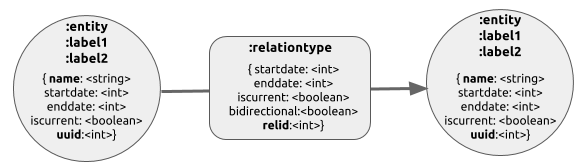
\includegraphics[width=1\textwidth]{model1} 
\caption{Generic model - two entities with a relation}
\label{fig:model1}
\end{center}
\end{figure}

\begin{figure}[H]
\begin{center}	
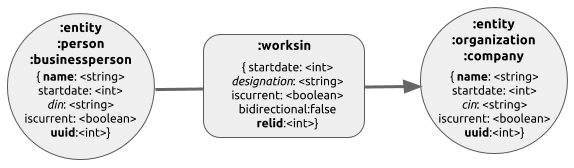
\includegraphics[width=1\textwidth]{model2} 
\caption{A model showing businessperson- organization relationship }
\label{fig:model2}
\end{center}
\end{figure}

\begin{figure}[H]
\begin{center}	
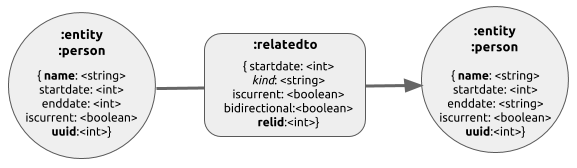
\includegraphics[width=1\textwidth]{model3} 
\caption{Model showing person-person relationship}
\label{fig:model3}
\end{center}
\end{figure}

\begin{figure}[H]
\begin{center}	
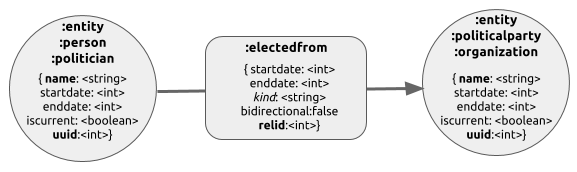
\includegraphics[width=1\textwidth]{model4} 
\caption{Model showing politician - party relationship }
\label{fig:model4}
\end{center}
\end{figure}

\begin{figure}[H]
\begin{center}	
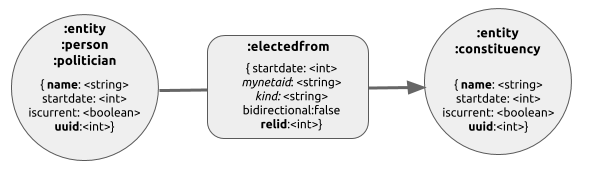
\includegraphics[width=1\textwidth]{model5} 
\caption{Model showing politician  - constituency relationship}
\label{fig:model5}
\end{center}
\end{figure}

\begin{figure}[H]
\begin{center}	
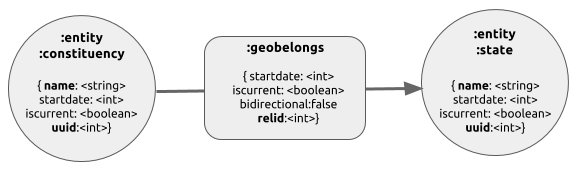
\includegraphics[width=1\textwidth]{model6} 
\caption{Model showing relation between person and his home state}
\label{fig:model6}
\end{center}
\end{figure}

\begin{figure}[H]
\begin{center}	
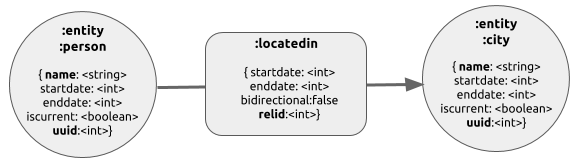
\includegraphics[width=1\textwidth]{model7} 
\caption{Model showing relation between person and his home city}
\label{fig:model7}
\end{center}
\end{figure}

\begin{figure}[H]
\begin{center}	
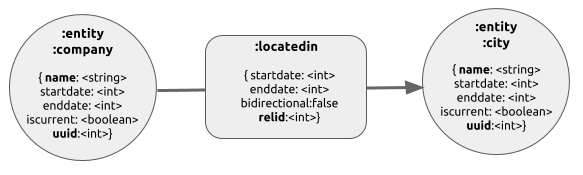
\includegraphics[width=1\textwidth]{model8} 
\caption{Model showing relation between organization and its home city}
\label{fig:model8}
\end{center}
\end{figure}

\begin{figure}[H]
\begin{center}	
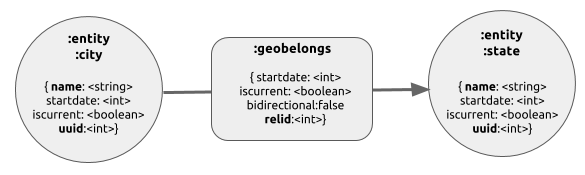
\includegraphics[width=1\textwidth]{model9} 
\caption{Model showing city-state relationship}
\label{fig:model9}
\end{center}
\end{figure}

\section{Data collection and description}
\label{datacollect}

Since the aim was to to build a social network for all the Indian power houses, we needed to identify and collect as much varied data as possible. It is only when different kind of data mingle with each other in the system that we can hope to see some hidden patterns or dig out interesting insights. All the visualizations that we obtained from this data are shown in the analysis Chapter \ref{chapviz}

We needed to search for alternate data sources that might help the ongoing work. We have looked for datasets spanning company details, board of directors, Lok-Sabha MPs, subsidiaries, banks, and any other relevant political-corporate data. 

Any data that is crawled is not fed into the system directly. Instead, a REST PUSH API provided by our system is used to push it to a separate crawl data-store (rather than the core data-store) for moderation first. The  data integration is described in next section, while the REST API is described in next chapter. 

\subsection{Challenges}

\begin{enumerate}

    \item  The biggest challenge in data collection is that data for Indian context is not easily available.  Open data initiatives like data.gov.in have initiated hope for data enthusiasts but there is still a long way to go. 

    \item No central place for any category of target data, so one would have to look for multiple sources. Instead, in a way, we are striving to create such a central place in the present work.

    \item Since data has to be integrated from variety of source points, the credibility of a data item listed can be established strongly but with the added evil of entity resolution - which has been explained in a later section. 

    \item Mostly, no unique identifiers for entities appear in datasets that are publicly available. There is a possibility of duplication of data, this is where the ER work comes in handy.  

    \item Most data contained noise, or erroneous details at times. This sometimes is intentional on the data entry operator's part, sometimes it's just a naive mistake. For example: name for some people was wrongly spelt in some publicly available websites.

    \item Data was missing for some datasets. For example, in the affidavit that the politicians have to fill before elections, or in the data collected from companywiki.

    \item Names are the biggest problems in such a work. People use titles like Mr., Shri, Shriman, Late, Lt., Mrs., Kumari, Kumar which again add more complexity to the problem. 

    \item There is no standard data format for dates even across government departments. Similarly for the address - there is no standard format to extract out relevant information.

    \item Most of the government sites maintain significant data on-line but hidden in a complex web of links and most of the times the data is available as PDF files.


\end{enumerate}


\subsection{Tools and Methods}

We describe here tools that we picked and methodology adopted up along the way for data collection and cleaning. It is important to note that no single tool can be a cure for all the data-sources. In fact, what we have learned in due course of time is that different kind of data sources require different approach.
The data being noisy due to entry errors and the schema/ model/ format differences of the sources causes various consistency issues to creep up when compiling them into a single model.
There are other issues of not obtaining enough data to churn out any useful information. In that case we have adopted techniques of generating more data from that which is available.

\begin{enumerate}

    \item A \textbf{ naive method } that we experimented during the initial work is to fetch an html page through python's urllib library, and then parsing the same with BeautifulSoup library. Advantages of Beautiful soup is that it allows users to get html elements by text query instead of div ids like xpath or css selectors. On the downside, this approach requires all cases of failures handled explicitly in the code. Even the data to be stored is to be explicitly written in desired type of file (csv in our case).

    \item \textbf{ Selenium } - It is basically a web testing framework, mainly used to automate human interactions with an website. Running Selenium is similar to having an human agent using a browser to select items and extract data for you. Since it works as an agent with a browser, many issues get automatically averted like - authentication issues against a bot, easy interactions with browser gui elements (for eg. - modal panes) etc. Selenium was extensively used in scraping of the companywiki website.

    \item \textbf{ scrapy } - scrapy is a framework to create a web crawler bot which can be used to crawl the web and scrape pages. It has almost everything required to get data easily. A request wrapper to send requests at ease, callback functions to handle errors, ORMs to store the data with ease with whatever format user wants, file down-loader etc. scrapy also uses twisted, an asynchronous network library which is event driven. So unlike other tools above, data collection with scrapy is very fast. The disadvantage however is that of a high learning curve which can be a waste of time if amount of data to be collected is not that high. Scrapy also cannot interact with same page Javascript requests and interact with browser elements. The websites of Loksabha, RajyaSabha were scraped using scrapy.

    \item \textbf{ Manual data collection } - When the dataset is small, it is manually collected by using some tool ( Google sheet's \emph{ ImportHtml } function for example) or by simply doing data entry by hand. The resultant data is free of errors with some trade-off for time. Manual work is also required when \textbf {\emph { bootstrapping some dataset } }. Bootstrapping is the process of expanding a dataset using some seed dataset. For our case, we collected data for top 1000 companies by value. From this initial seed, company id no. (CIN) was collected from companywiki site, with their director information. Finally director's pages were looked after to collect information about other companies owned by them. In the end, this data generated a total of 60000 company records.

    \item The \textbf{ data collected is preprocessed } using the python pandas library. Here issues like encoding mismatch (\emph{ utf-8 vs ascii }), text format conversions (like \emph{ converting a date given in string to UNIX timestamp format }) and text normalizations ( like \emph{ name field reduction to FirstName\textless single space \textgreater LastName }) are handled .

\end{enumerate}


\subsection{Corporate data}

The challenges in collecting any corporate data are:

\begin{enumerate}
    \item Getting government provided unique identification numbers for the company
    \item Getting government provided director identification numbers for their directors
    \item Linking these two IDS.
    \item Getting the list of all companies over the time with their Ids of course.
    \item Getting the list of subsidiaries for each company/group. (The toughest job)
\end{enumerate}  

We have been able to tackle the first four challenges to a commendable extent but the last one.  We first describe the sources we have encountered, and finally how we collected our corpus of 90000 directors and 60000 companies.

% A related work is Parag's [citation]. 


\subsection{Ministry of Corporate Affairs (MCA)} 

Being the official government source, MCA \cite{MCA} is the most authentic data source we have found for obtaining the list of companies and LLPs (Limited Liability Partnerships) operating in India. It gives us all the companies registered year-wise before and after 1980 till date in the form of pdfs with their CIN/LLPIN (Corporate Identity Number/Limited Liability Partnership Identification Number) which is unique to a company/LLP. The only downside as always with any pdf data is a lengthy parsing job.

MCA, with its search engine, contains a huge amount of data. Armed with the CIN, we can obtain a lot more information for a company from the MCA site itself. We get the type of the company, the category of the company, the headquarters, its market capital, date of incorporation and the charges it is facing. Not only that we also obtain the signatories of a company from the MCA site as well i.e. their board of directors, with their unique DIN(Director Identity Number). This can again be useful in entity resolution. (This is a new feature they introduced).

But MCA with all its data poses a lot of problems to deal with-
\begin{enumerate}
    \item MCA has an exhaustive list of all legally registered companies which is a really big number to process. As such, not only crawling  them will be a lengthy task, but also processing the data after crawled and filtering out the relevant companies of interest. Then will come the issue normalizing and cleaning up the data.
    \item Crawling MCA and scraping it is not a very straight forward task as the web UI within it contains a bad control flow with  manipulation of many browser GUI elements which as of now can be performed by testing frameworks like Selenium only. This is a real performance bottleneck determined by speed of Selenium and MCA server. 
    \item Although it allows one to look for director DINs and other information from a CIN, the reverse is not implemented. The site does not also provide enough filtering options to filter out data in first place.
\end{enumerate}

\subsection{Initial approach, Capitaline database and CompanyWiki}

Initially we tried to collect company data by searching the names of politicians as potential directors. This helped us to find companies associated with politicians as source of potential overlap between coporate-politcians. But the problem was that most of the companies that the politicians are linked to are small businesses on which we have little interest. Thus, we changed our approach to obtain the companies of interest (most valued companies for example), and find the entities linked with them. These entities of the top companies are actual power elites by our definition. Any links between them and politicians (direct or indirect) are our actual point of interests.
At this juncture, we utilized the data from \textbf{Capitaline} \cite{capitaline}. Capitaline is a database containing info on Indian companies. 

% We used Capitaline data as collected by Parag Pahwa[citation].

The data collected consisted of following information-
\begin{itemize}
    \item Company name
    \item Director
    \item Subsidiaries, if any
    \item Values in crores
    \item Donations to political parties
\end{itemize}

However, the problem was that it had no unique ids like CIN, DIN to uniquely determine a company or director and help us in resolution. So we decided to generate a new dataset of our own. Using the Company Name and Value field we picked top 1000 valued company and looked for relevant information in other data stores like CompanyWiki. 
CompanyWiki is another website containing data from mostly MCA. It helped us by giving a better platform with more options of searching/ querying the data. It also contained government IDs for the entries (CIN for companies, DIN for directors etc. ) which helped us to link entities. The website also allowed us to search on CINs, DINS  / get CINs given DINs and vice-versa. 
For our purpose we obtained our director sharing data by following means-

\begin{enumerate}
    \item Obtain top 1000 valued company from Capitaline data - an SQL query on database table storing the company name and value ordered by value and limit to 1000 entries.
    \item Manual annotation of 1000 companies to get its CIN. This was done by searching for the company name in CompanyWiki.
    \item Running Selenium script for taking the list of IDs to get all director names, DINs from CompanyWiki.
    \item Using these to get all the companies, CINs where the corresponding director is a member. Here also Selenium was used to get the company names, CINs from the list of DINs inputted. The script took entire 3 days to complete the task. Advantage of using the CIN here became useful when duplicates are filtered with the help of it.
\end{enumerate}

Thus in this way a dataset of 1000 companies and  9400 directors were expanded to a dataset of 90000 directors and 60000 companies. This data formed the starting point in our Core Database.

\subsection{Political data}

Our task in this domain was to find personal information of MPs and their dependents. So we went looking in Wikipedia of various political members and their families. But Wikipedia is highly unstructured and crawling, parsing Wikipedia even with professional extractors is a tedious task.

We started with these problem statements in our mind:
\begin{itemize}
    \item How to get info on all 16 Lok Sabha's MPs?
    \item How to get the family information of MPs?
\end{itemize}
\subsection{MyNeta}
MyNeta is a site launched by Association of Democratic Reforms (ADR) to provide public awareness about Indian politicians. They contain several important information about Indian MPs including -
\begin{itemize}
    \item Personal information
    \item State, Constituency of MP
    \item Assets and Liabilities
    \item Criminal cases - if any
\end{itemize}
For our work, we used only the personal information of the politician. MyNeta also keeps an internal id (named MyNeta ID) which we keep to resolve duplicates in the data.

\subsection{Lok Sabha Official data}

We also chose to scrape official LokSabha site for politician's personal properties as per government records for better triangulation of political entities (especially when we found some information missing in MyNeta dataset) and also for looking up family ties of the political leaders.
We finally got this information from official site of LokSabha which gave us actual government provided records. Scripts were written in scrapy which allowed us to gather information about politician. We also downloaded the images of politicians to be used later in the Power Elites web app \ref{chapwebapp}.

\subsubsection{Rajya Sabha Official data}

We collected Rajya Sabha data as well from their official site to look for more corporate-political tie ups. Rajya Sabha data is more interesting as we have some businessmen directly nominated as a Rajya Sabha.  

\section{Family Ties Information}

We also have manually collected from the web various family ties in businesses and politics. Major source for this data is wikipedia. This data allowed us to find new relations/links from already obtained graph.\cite{indianbfamilies} \cite{indianpfamilies}


All the mash-ups created by these datasets have been reported in viz section \ref{chapviz}

\section{Data integration}
\label{dataint}

As discussed earlier, the real challenge of forming a data mashup is the non-uniformity of different sources which include differences in schema, data model, formats of text, assumptions of persons scraping the data(hereby referred to as \textbf{ data gatherers } or \textbf{ gatherers }) etc. To alleviate such problems, we came up with a particular data format to be used by all data gatherers on conformance with which he or she should pre-format the data before pushing in to the system. By separating out the problem of data integration, we have reduced maintenance costs for the knowledge base. In this way, the schema described in the system model is kept intact, while the data gatherer can crawl the data by his own whim as long as he conforms to the data format expected by the write API.

The initial plan was to allow the crawled data to be pushed into some MySQL database. Each gatherer would then have to define a mapping somewhere to map all the fields of the crawled data to the fields in the actual graph data. But this poised the problem of maintaining a new map file/table which was crucial to data pushing. The data gatherer would have to enlist new mappings for every new data crawled from a source. The maintenance of the  would have been another problem to deal with.
%
Instead we chose to provide gatherers with a REST API and  a specific data format which he/she has to adhere to while pushing in the data.
For now, JSON payload is used in a specific format. Similar to the graph database format, this payload is designed as follows -

\begin{lstlisting}[language=json,firstnumber=1]
{
    "taskid": "1",
    "userid": "abhi2@gmail.com",
    "token": "jhfhybfdkjfygfjk87gdfgdjf5",
    "entities": [{
        "id": "1",
        "fetchdate": "1466024344",
        "sourceurl": "http://loksabha.nic.in",
        "labels": ["person", "politician", "entity","businessperson","memberofParliament"],
        "properties": {
            "name": "Naveen Jindal",
            "address": "Kurushetra",
            "dob": "11 Feb, 1970",
            "job": "business"
        }
    }, {
        "id": "2",
        "fetchdate": "1466024344",
        "sourceurl": "http://loksabha.nic.in",
        "labels": ["organization", "politicalparty", "nationalparty", "entity"],
        "properties": {
            "name": "Indian National Congress"
        }
    }],
    "relations": [{
        "id": "1",
        "label": "memberof",
        "start_entity": "1",
        "end_entity": "2",
        "fetchdate": "1466024344",
        "sourceurl": "http://loksabha.nic.in",
        "bidirectional": "no",
        "properties": {
        }
    }]
}
\end{lstlisting}

The main components of the payload is as follows -
\begin{itemize}
    \item entities - array with each element having following info
        \begin{enumerate}
            \item id - unique id specific to data gathering task
            \item labels, properties - adhering to an entity in graph db
            \item sourceurl, fetchdate - to be used for provenance (to be given by the gatherer) to be discussed in chapter \ref{chapwebapp}
        \end{enumerate}
    \item relations - array with each element having following info
        \begin{enumerate}
            \item id - unique id specific to data gathering task
            \item startentity,endentity - ids of entities
            \item isbidirectional - whether the relation is bidirectional 
            \item labels, properties - adhering to relation properties in graphdb
            \item sourceurl, fetchdate - to be used for provenance (to be given by gatherer) to be discussed in chapter \ref{chapwebapp}
        \end{enumerate}
    \item authentication info - used by the Power Elites app described later \ref{chapwebapp}
\end{itemize}

All data crawled or manually collected is first pushed into a separate graph database ( a separate Neo4j instance)-  \emph{ "crawl data store" } (here onwards refer to as crawl-DB) using REST API calls with the JSON payload. The pushed data is then verified/resolved by human moderator before being pushed to the system. A high level view of the central internals of the system is shown in the Figure \ref{fig:twodb}.

\begin{figure}[H]
\begin{center}  
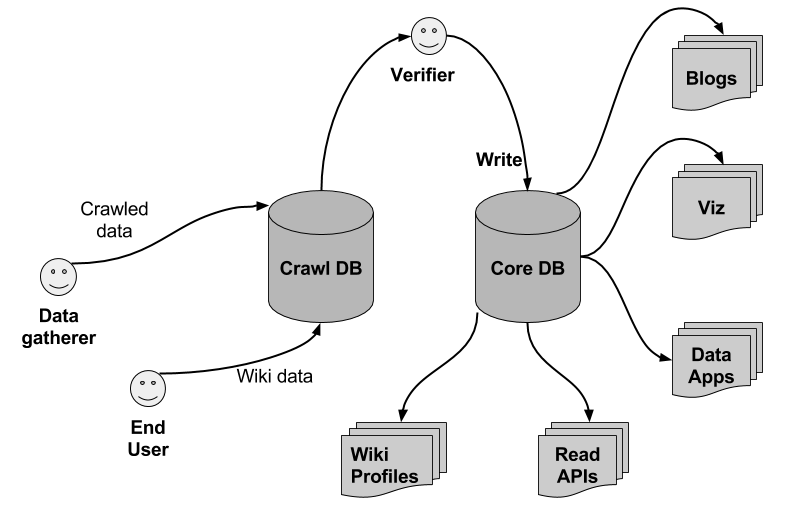
\includegraphics[width=0.7\textwidth]{twodb} 
\caption{A basic model of the system}
\label{fig:twodb}
\end{center}
\end{figure}

This way - we will have different non-connected subgraphs in the Crawl - DB .  
But how do we resolve the nodes and relations now with the core data store? The basic setup id described in the next section. 

\section{Entity Resolution}
\label{dataer}

The basic algorithm of entity resolution goes as follows-

\begin{algorithm}[H]
\KwData{Datasets - S, T }
\KwResult{list -L consisting of proper matches of T in S }
initialization - L is empty \;
parameters - S,T, threshold \;
 \For{all records t in T}{
  \nl search for t in S \;
  \nl pick records s in S for which match-score(t, s) $\geq$ threshold \;
  \nl append all s in L \;
 }
 \caption{Generic Entity Resolution}
\end{algorithm}

Complexity of above algorithm is O(n*m) where n is size(S) and m is size(T) when n records are searched linearly in S.
        From the above, we can find that the two crucial operations here is the choice of proper scoring algorithm to pick s in line and search of t in S in line 1.

\section{String Matching Algorithm}
        The requirement of a scoring algorithm was such that it should match words with small spelling mistakes and similar names. In our case, we have used Jaro-Winkler distance as it considers ranges and transpositions while matching two words. A sample experiment from our side on a list of four names showed the scores as seen in table \ref{table:1}.
    \begin{table}[H]
    \centering
    \caption{Comparison of string matching algorithm}
    \label{table:1}
    \begin{tabular}{|l|l|l|l|l}
    \cline{1-4}
    \textbf{Words}                   & \textbf{levenshtein} & \textbf{jaro\_distance} & \textbf{jaro\_winkler} &  \\ \cline{1-4}
    vidya vs biday                   & 3                    & 0.78                    & 0.78                   &  \\ \cline{1-4}
    saawan kumar vs saavn kumer      & 3                    & 0.86                    & 0.89                   &  \\ \cline{1-4}
    gautam adani vs gautambhai adani & 4                    & 0.86                    & 0.92                   &  \\ \cline{1-4}
    \end{tabular}
    \end{table}
        Upon a test run of all algorithms over a sample of 100 names from our datasets we decided to use jaro-winkler for the purpose. We also required to match names which are phonetically similar to other names. These helped us to match names like \textit{ 'Gautam' } and \textit{ 'Gautambhai' }, \textit{ 'Vidya' }, \textit{ 'Bidya' } and \textit{ 'Biday' } etc.

\section{Comparison techniques}
        As obvious from above algorithm the performance of entity matching algorithm depends largely on how fast the searching occurs in dataset S. A naive algorithm like above added a factor of O(n) on linear search over entire S. As a result, the performance of the entire system got bottlenecked by the resolution module. As a result we sought out for other solutions regarding this. The obvious improvement over it is the possible implementation of a binary search to reduce search speed to O(log n) time. But binary search is not applicable here for following two reasons -
            \begin{enumerate}
                \item Binary search uses a predicate like gt, eq, lt , the value of which is true or false. Such predicates determines some order in the dataset. 
                \item The absence of such predicates as above avoid any sorting or ranking of the data in any order for any possibility of binary search.
        
            \end{enumerate}

\section{Machine learning techniques}

        After having performance bottleneck in searching records in other datasets, we looked for probabilistic ways of solving the same problem. We used the python library of dedupe \cite{dedupe} for this purpose. The library basically induced an active learning mechanism to obtain training samples where it picked two entities of possible match and prompts the user to label positive/negative. It then matches the related entities accordingly with the hypothesis formed. Unfortunately this approach suffered from following drawbacks-
        \begin{itemize}
        \item Too small data to accurately form a proper hypothesis. 
        \item The labels that were asked to mark along with data were picked at random and often the results of the algorithm are different in different runs (depending on the number of positive or negative label given at that time).
        \end{itemize}
        Fortunately indexing other dataset helped to come out of this.

\section{Indexing and Apache Solr}
        Indexing allows searching to be very fast of near O(1) speed. Indexes are data-structures that store contents of a document (in our context fields of records in a dataset) for faster access to the document. This enables faster retrieval with a trade off for using more memory. For our purpose we used Apache Solr framework \cite{solr}for the searching step. Solr uses Apache Lucene \cite{lucene} to create an inverted index based desired on fields in the records. An inverted index basically creates a data structure on the content of the records and have pointers to the actual locations of the records. So for all text in the specified fields, Lucene breaks them (tokenizes them) and store them in a data structure for fast retrieval.  Solr also sets up a  Web server with REST APIs to allow us to integrate it with other parts of our system described in Chapter \ref{chapwebapp}. 
        Since Solr has its own sets of protocols we had to modify the way we apply the resolution algorithm described above. The main steps followed by us to realize this are as follows.\cite{solrdocs} 
\begin{itemize}

        \item \textbf{ Defining a data set } to index  (the data set S above). We described a data source which contained the dataset. In this case, it was a mysql database. (file \emph{ db-data-config.xml }) .
        \item \textbf{ Defining the fields } to index. Solr needs to have a schema of the records to know which fields will indexed and which one is kept as satellite data. These are specified in solr configuration files. (file \emph{schema.xml})
        \item \textbf{ Defining how to preprocess } all the terms before creating the index. Solr allows to specify a list of pre-built tokenizers, stemmers, filters to preprocess a term or custom ones if necessary. We used whitespace tokenizers and double metaphone phonetic filters to get a match score relevant to our purpose and in this way used the phonetic algorithm for better text matching. (file - \emph{ solrconfig.xml })
        \item \textbf{ Forming a lucene query } based on the contents of records of another dataset (data set T above)
        \item \textbf{ Applying Jaro algorithm } for comparison was difficult in Solr. This is because, all the functions applied to the text for indexing are necessarily single parameter. Jaro or any other non-phonetic string metric needs at lest two string Results returned by the Solr is further filtered by the Jaro-Winkler algorithm. Results being quite small, does not take much time even if a one-one matching algorithm is executed. 

\end{itemize}
\subsection{Solr Fields}
    To effectively triangulate two entities, special emphasis was given on which fields to compare while doing it. After few experiments we decided to match records on following fields generated from the graph data model we discussed in previous section.

\begin{itemize}
    \item \textbf{ Aliases }- a list that contains names pertaining to an entity. This is especially required when a person/institution is known by several names in the world. Eg. - Narendra Modi vs Narendra Damodar Modi, BJP vs Bharatiya Janata Party 
    \item \textbf{ Aliases  Phonetic } - same as above but here search is done on phonetic index.
    \item \textbf{ label } - Label dictates the type of entity as per data model in section- \ref{datamodel}.
    \item \textbf{ Keywords } - a list that contains main keywords of the entity. This field is most helpful in triangulation as it indexes all the properties of the entity and the aliases of the entities directly related with the original entity. Important properties unique to a particular entity like location for a particular item.
\end{itemize}

\subsection{Lucene Queries}
    Proper search queries are essential to efficiently resolve an entity. These involved using above fields effectively to obtain relevant entities- 
    The grammar of the lucene query used by us goes as follows-\\
        \emph{ \textbf{ L } ::=   \textbf{ I }':'(\textbf{Q}) \textbf{L}  OR $\epsilon$ } \\
       \emph{ where,  \textbf{I} ::= \textless index field \textgreater  }\\
        \emph{ \textbf{Q} ::= \textless query string\textgreater to be matched against I } \\

    query string can be as follows -\\
    
    \emph{ "string text" } - matching the exact word 'string text'\\
    \emph{ string text } - matches string or text or both \\
    \emph{ string$\sim$ } - lucene applies edit distance to string and returns the possible matches \\
    
    %The query we used for our purpose is as follows-
    %" labels:(each label separated by whitespace) aliases:(each alias~ separated by whitespace ) AND aliases-phonetic:(each alias separated by whitepace) AND keywords:( each keyword~ separated by whitespace)"
    More details on lucene query can be found at \url{https://lucene.apache.org/core/2\_9\_4/queryparsersyntax.html}
    %Eg. - 
\subsection{Performance}
    On testing our Solr integrated system with the original basic resolution algorithm, we found many fold improvements. Initially upon resolving 1000 corporate entities against about 500 political ones over the "name" field in both took us about 150 minutes to resolve. That makes resolution of a single entity about 18s.
    Compared to that, a single entity is resolved in Solr in little over 1s showing a performance upgrade of about 18x.

